\newpage
\section{Durchführung}
    \subsection{Versuchsaufbau}

        \FloatBarrier

        \begin{figure}[h]
          \centering
          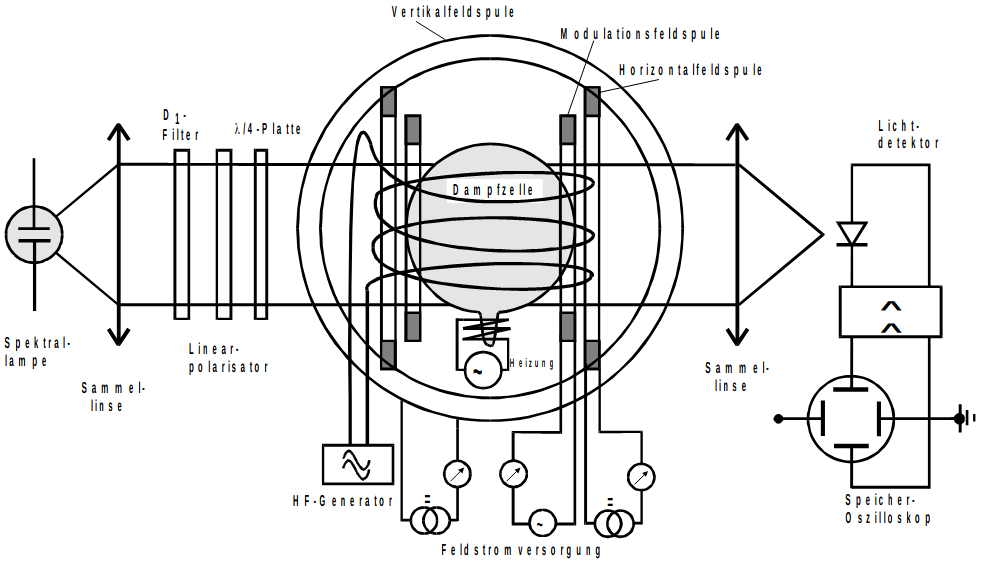
\includegraphics[width = 0.6\textwidth]{pictures/Aufbau.png}
          \caption{In der Abbildung ist der schematische Aufbau der gesamten Messapperatur dargestellt. [1]}
          \label{fig:Aufbau}
        \end{figure}

        \FloatBarrier

        \noindent
        Wie im schematischen Aufbau zu erkennen, wird das Licht der Spektrallampe zunächst kollimiert und dann auf eine Wellenlänge von \SI{794.8}{\nano\metre}. Daraufhin wird es zunächst linear und anschließend 
        durch einen $\lambda$/4-Filter zirkular polarisiert. Nach Durchlaufen der Dampfzelle wird das Licht durch eine weitere Linse auf einen Photodetektor fokussiert, der sein Signal an ein Oszilloskop 
        weitergibt. Die Gaszelle selbst wird bereits vor dem Versuch auf circa 100° erhitzt, damit das Rubidium vollkommen gasförmig vorliegt. Um die Gaszelle sind eine horizontale und eine vertikale Spule 
        angebracht, die die jeweiligen Komponenten des Erdmagnetfeldes komprensieren sollen. Zusätzlich ist in horizontaler Richtung eine Sweep-Spule angebracht, die in der Lage ist einen vorgegebenen 
        B-Feld-Bereich zu durchlaufen. Die letzte Komponente ist ein Hochfrequenz-Generator, der ein Radiofrequenz-Feld innerhalb der Dampfzelle erzeugen kann.

    \subsection{Kompensierung des Erdmagnetfelds}
        Zu Beginn der tatsächlichen Messreihen soll keine Zeemann-Aufspaltung vorhanden sein. Dazu muss das Gesamtmagnetfeld innerhalb der Dampfzelle gleich null sein. Um dies zu überprüfen, wird die Intensität
        der durch die Dampfzelle tretenden Strahlung gemessen. Wenn das Magnetfeld gleich null ist, verschwindet die Zeemann-Aufspaltung und die Intensität sinkt, da die Absorption steigt. Nun wird der 
        Strahlengang mit Hilfe eines Kompass entlang des horizontalen Erdmagnetfelds ausgerichtet und die Spannung der horizontalen Spule so angepasst, dass die Intensität minimal wird. Daraufhin wird auch die
        Spannung der vertikalen Spule angepasst, bis die Intensität minimal ist. Nun ist auf dem Oszilloskop ein schmaler Dip zu sehen und es kann mit der eigentlichen Messungen begonnen werden.  

        \FloatBarrier

        \begin{figure}[h]
          \centering
          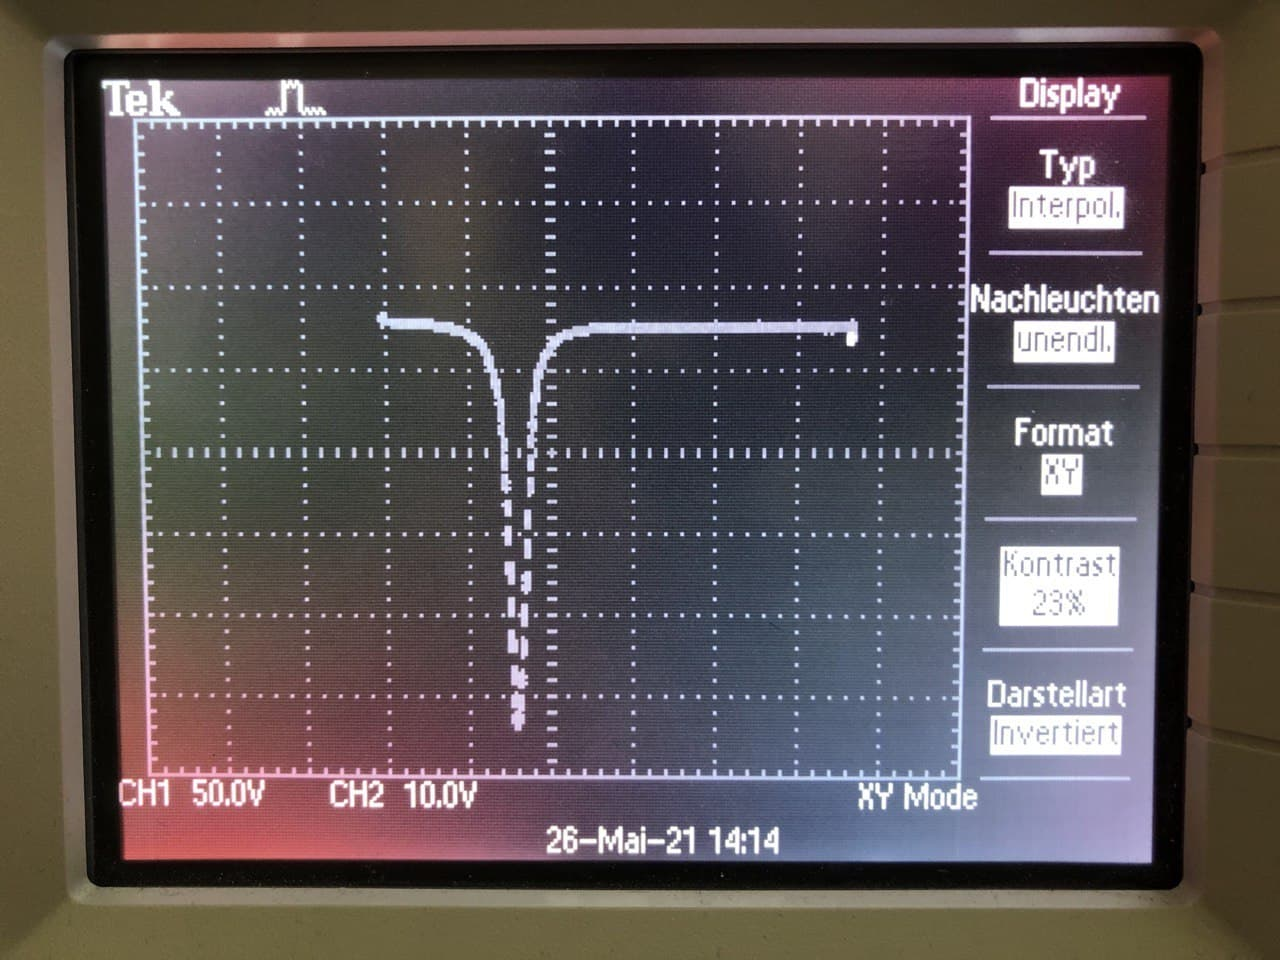
\includegraphics[width = 0.6\textwidth]{pictures/B_0.jpg}
          \caption{In der Abbildung ist der Dip auf dem Oszilloskop zu sehen, der dadurch entsteht, dass annähernd das gesamte Erdmagnetfeld innerhalb der Gaszelle kompensiert wird. [1]}
          \label{fig:B_0_dip}
        \end{figure}

        \FloatBarrier

        \noindent

    \subsection{Messung des Zeemann-Effekts}
        Um den Zeemann-Effekt zu messen wird zunächst ein äußeres RF-Feld angelegt. Dann wird die Sweep-Spule aktiviert, die einen vordefinierten Bereich des B-Feldes durchläuft. An den Stellen, wo die 
        Zeemann-Aufspaltung durch das B-Feld der Energie der Photonen des RF-Feldes enstpricht, kommt es wieder zu einem Dip der Intensität. Da die Dampfzelle zwei Rubidium-Isotope beinhaltet, kommt es auch zu 
        zwei Dips. Diese Dips werden genauer untersucht und es wird die Spannung der horizontalen und die der Sweep-Spule abgelesen, um später das der Zeemann-Aufspaltung zugehörige B-Feld zu bestimmen. Diese 
        Messung wird in Schritten von \SI{100}{\kilo\hertz} im Bereich zwischen \SI{100}{\kilo\hertz} und \SI{1}{\mega\hertz} der RF-Frequenz wiederholt. 

        
        
